% Method overview (Fig. 6). Compile with pdflatex; drawn at print size (12.9 cm wide), sans-serif type.
\documentclass[border=2pt]{standalone}
\usepackage[T1]{fontenc}
\usepackage[scaled=0.95]{helvet}
\renewcommand{\familydefault}{\sfdefault}
\usepackage{tikz}
\usetikzlibrary{positioning,arrows.meta}
\begin{document}
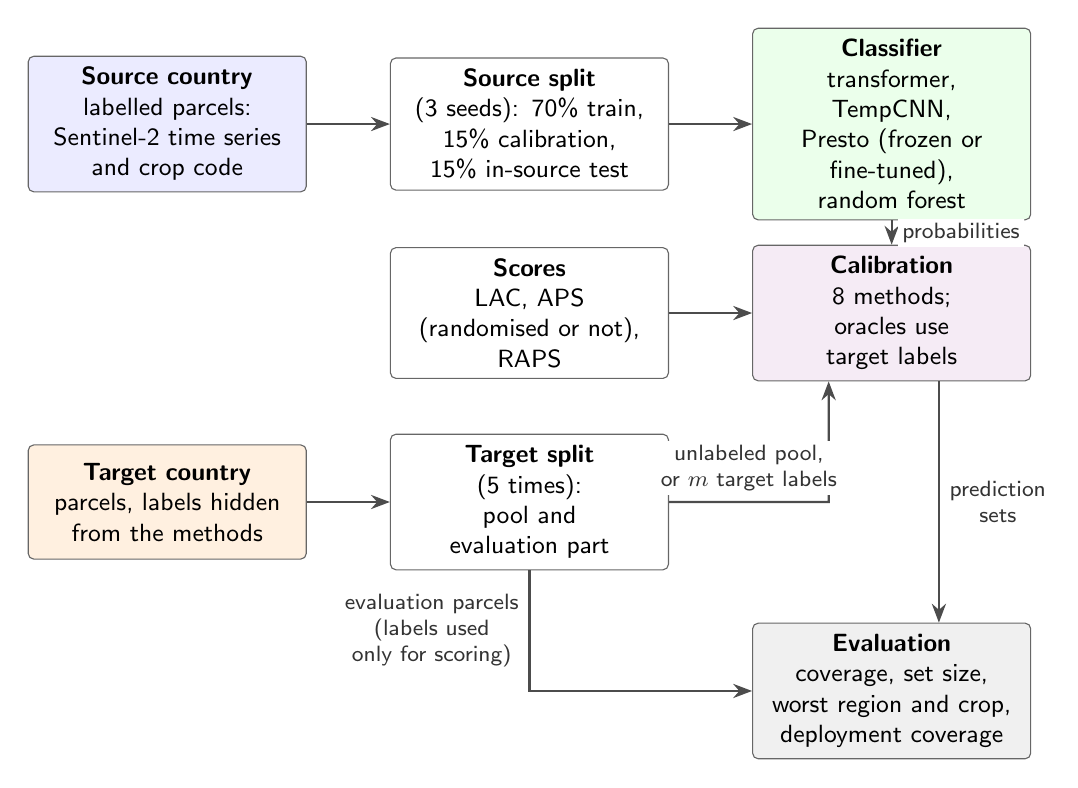
\begin{tikzpicture}[
  box/.style={draw=black!60, rounded corners=2pt, align=center, font=\small, inner sep=4pt,
              minimum height=1.45cm, text width=3.25cm, execute at begin node={\hyphenpenalty=10000\relax}},
  arr/.style={-{Stealth[length=2.4mm]}, thick, black!70},
  lab/.style={font=\footnotesize, text=black!80, fill=white, inner sep=1.5pt, align=center}]
\node[box, fill=blue!8]   (src)    at (0,0)     {\textbf{Source country}\\labelled parcels:\\Sentinel-2 time series\\and crop code};
\node[box]                (split)  at (4.6,0)   {\textbf{Source split}\\(3 seeds): 70\% train,\\15\% calibration,\\15\% in-source test};
\node[box, fill=green!8]  (model)  at (9.2,0)   {\textbf{Classifier}\\transformer, TempCNN,\\Presto (frozen or\\fine-tuned), random forest};
\node[box]                (scores) at (4.6,-2.4) {\textbf{Scores}\\LAC, APS\\(randomised or not),\\RAPS};
\node[box, fill=violet!8] (calib)  at (9.2,-2.4) {\textbf{Calibration}\\8 methods;\\oracles use\\target labels};
\node[box, fill=orange!12](tgt)    at (0,-4.8)  {\textbf{Target country}\\parcels, labels hidden\\from the methods};
\node[box]                (tsplit) at (4.6,-4.8) {\textbf{Target split}\\(5 times):\\pool and\\evaluation part};
\node[box, fill=gray!12]  (eval)   at (9.2,-7.2) {\textbf{Evaluation}\\coverage, set size,\\worst region and crop,\\deployment coverage};
\draw[arr] (src) -- (split);
\draw[arr] (split) -- (model);
\draw[arr] (model) -- node[lab, right=2pt]{probabilities} (calib);
\draw[arr] (scores) -- (calib);
\draw[arr] (tgt) -- (tsplit);
\draw[arr] (tsplit.east) -- (8.4,-4.8) node[lab, pos=0.5, above=2pt]{unlabeled pool,\\or $m$ target labels} -- ([xshift=-8mm]calib.south);
\draw[arr] ([xshift=6mm]calib.south) -- node[lab, right=2pt]{prediction\\sets} ([xshift=6mm]eval.north);
\draw[arr] (tsplit.south) |- node[lab, pos=0.25, left=2pt]{evaluation parcels\\(labels used\\only for scoring)} (eval.west);
\end{tikzpicture}
\end{document}
